\section{Classification Definition}
Given a collection of records (a training set) where each record contains a set of attributes, the classification has to find a model for one particular attribute (the class) as a function of the values of other attributes.
The goal is for previously unseen records to have the class attribute assigned as accurately as possible.
A test set is used to determine the accuracy of the model. Usually, the given data set is divided into
training and test sets, with the training set, used to build the model, and the test set used to validate it.

\bigskip
\begin{figure}[H]
    \centering
    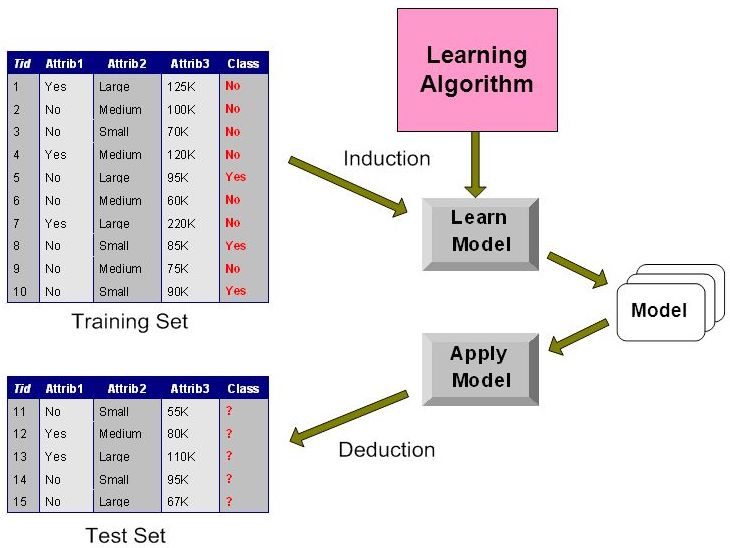
\includegraphics[scale=0.5]{figures/classification.jpg}
    \caption{Typical Classification Task}
\end{figure}

\subsection{Decision Tree}

A tree is built by splitting the source set, constituting the root node of the tree, 
into subsets, which constitute the successor children. 
The splitting is based on a set of splitting rules based on classification features. 
This process is repeated on each derived subset in a recursive manner called recursive partitioning. 
The recursion is completed when the subset at a node has all the same values of the target variable, 
or when splitting no longer adds value to the predictions. 
This process of top-down induction of decision trees is an example of a greedy algorithm, 
and it is by far the most common strategy for learning decision trees from data.

\medskip
Decision trees used in data mining are of two main types:

\begin{itemize}
    \item Classification tree analysis - When the predicted outcome is the class (discrete) to which the data belongs.
    \item Regression tree analysis - When the predicted outcome can be considered a real number.
\end{itemize}

\bigskip
\begin{figure}[H]
    \centering
    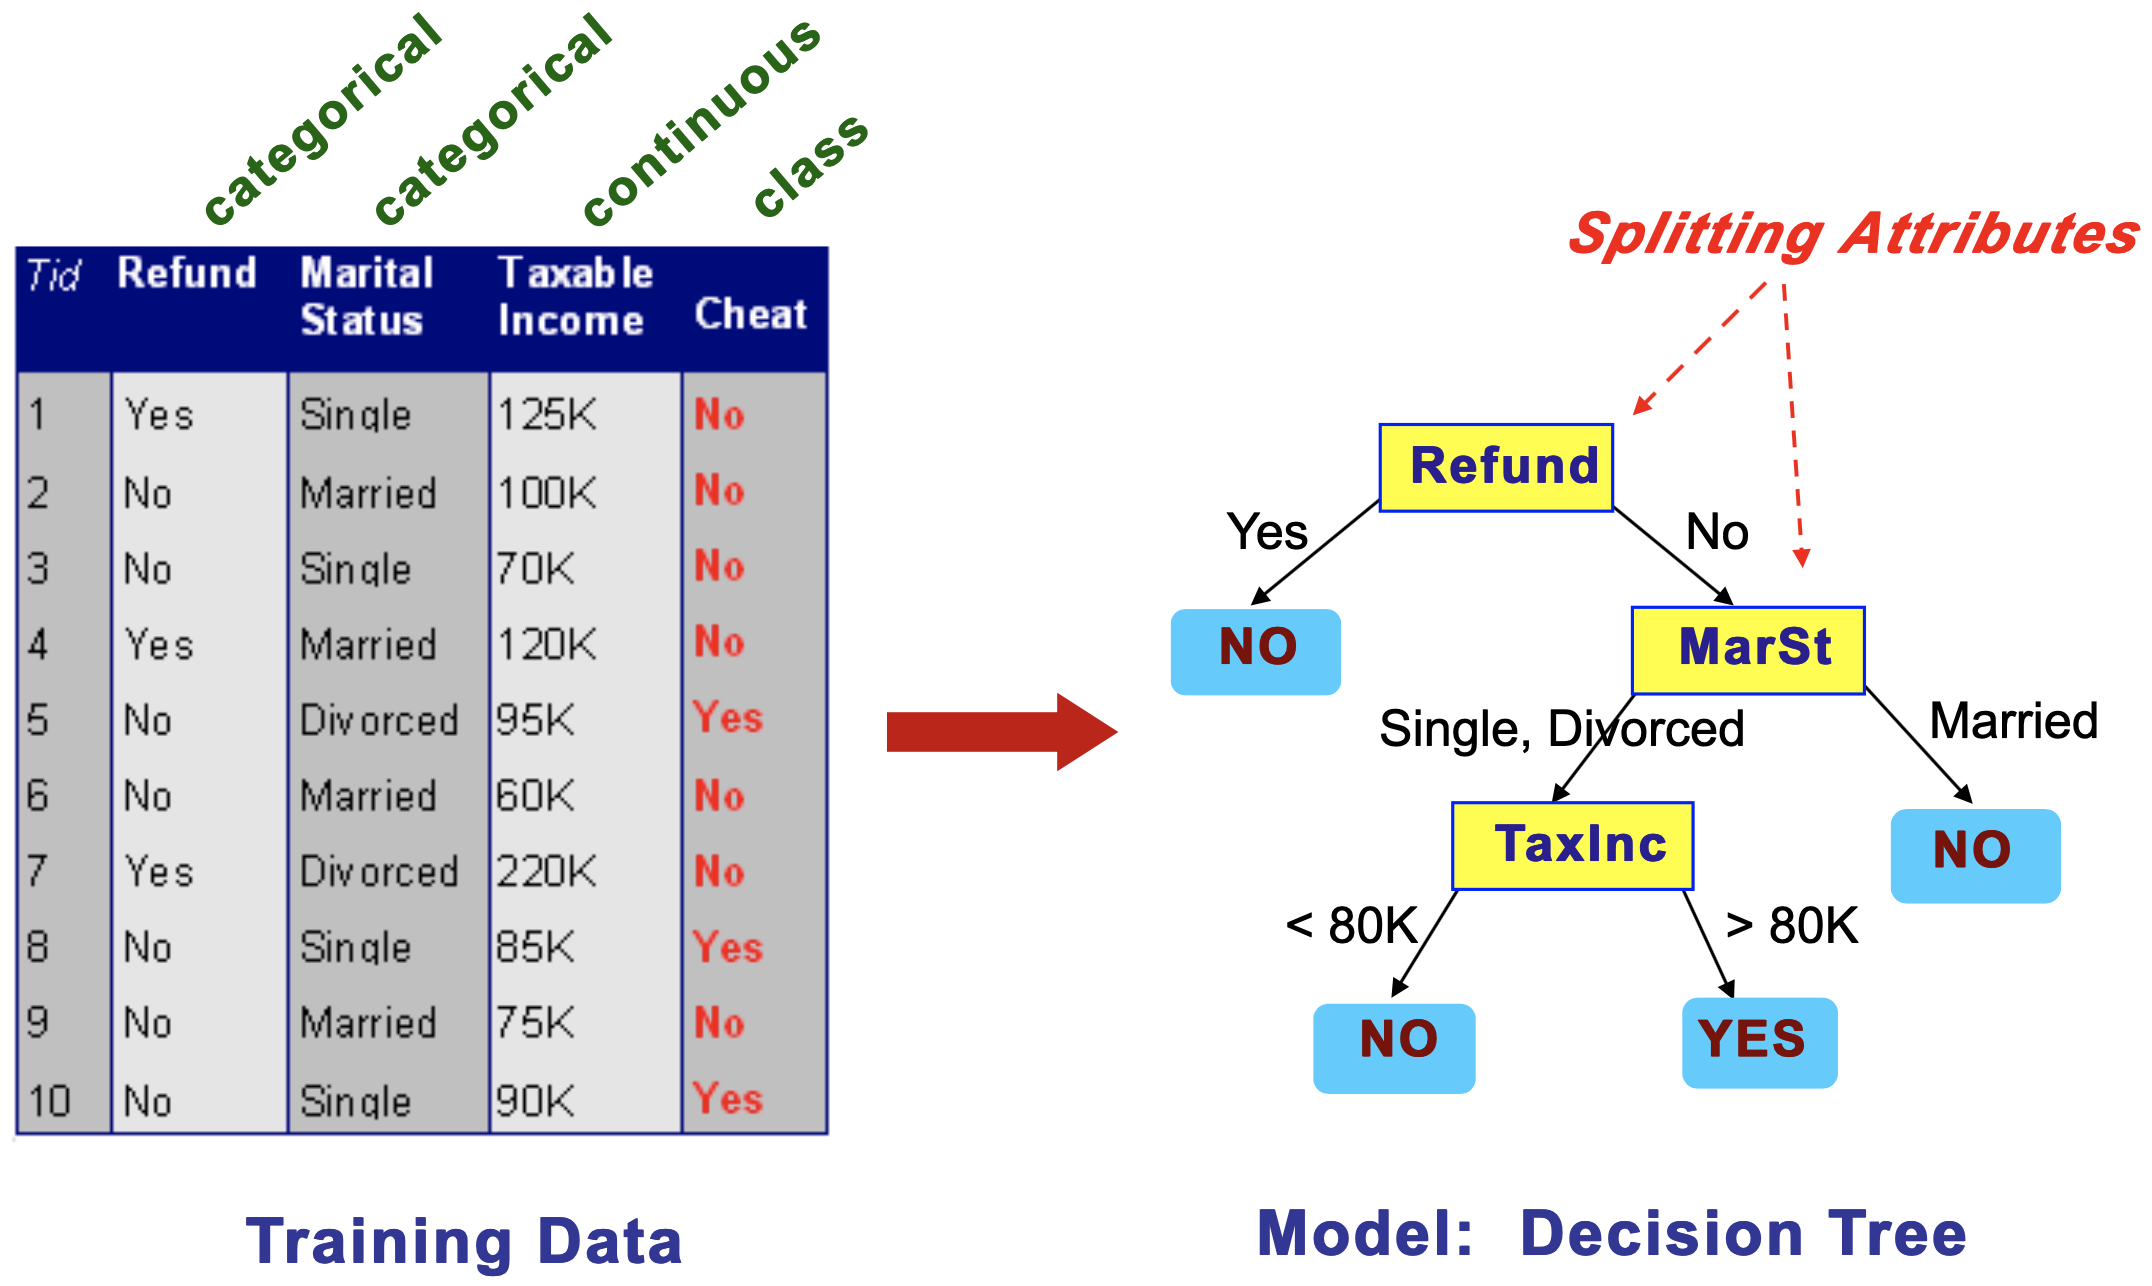
\includegraphics[scale=0.35]{figures/decisiontree.png}
    \caption{Typical Decision Tree}
\end{figure}

\newpage
\section{Hunt's Algorithm}

\begin{itemize}
    \item Let $D_t$ be the set of training records that reach a node $t$.
    \item General procedure:
    \begin{itemize}
        \item If $D_t$ contains records that belong to the same class as $y_t$, then $t$ is a leaf node labeled as $y_t$.
        \begin{itemize}
            \item This is a pure node.
        \end{itemize}
        \item If $D_t$ is an empty set, then $t$ is a leaf node labeled by the default class $y_d$.
        \item If $D_t$ contains records that belong to more than one class, use an attribute test to split the data into smaller subsets. Recursively apply the procedure to each subset.
        \begin{itemize}
            \item This is an impure node.
        \end{itemize}
    \end{itemize}
\end{itemize}

\section{Building Trees}
\subsection{Tree Induction}

The greedy strategy splits the records based on an attribute test that optimizes a certain criterion.

Issues with this approach include:
\begin{itemize}
    \item How to split the records. How should the attribute test condition be specified, and how is the best split determined?
    \item Determining when to stop.
\end{itemize}

\subsubsection{Specifying the Attribute Test Condition}
A proper test condition depends on the attribute type, which can be nominal, ordinal, or continuous.
\medskip

The condition also depends on the number of ways to split. This can be either a two-way split (binary) or a multi-way split. The binary split is often preferred as of the bushiness of the multi-way split. This means that very few records will match the leaf-nodes, and will therefore be overfitted.
\medskip

Ordinal attributes can be split the same way as nominal attributes, with some limitations if the order is to be preserved.
\medskip

For continuous attributes, there are two ways of handling splitting:
\begin{itemize}
    \item Discretization to form an ordinal catergorical attribute.
    \begin{itemize}
        \item Static - discretize once at the beginning.
        \item Dynamic - ranges can be found by equal interval bucketing, equal frequency bucketing, or clustering.
    \end{itemize}
    \item Binary decision.
    \begin{itemize}
        \item Consider all possible splits and find the best cut.
        \item Can be more compute intensive.
    \end{itemize}
\end{itemize}

\subsubsection{Determine Best Split}
When it comes to greedy approaches, nodes with a homogeneous class distribution are preffered.
\bigskip
\begin{figure}[H]
    \centering
    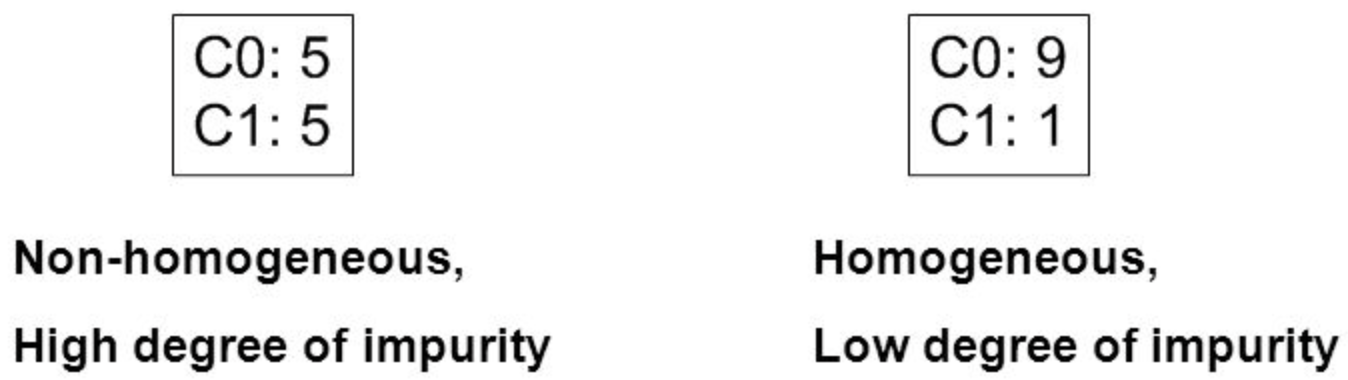
\includegraphics[scale=0.5]{figures/bestsplit.png}
    \caption{Class distributions}
\end{figure}

\section{Measures of Node Impurity}
Finding the best split follows closely to this process:

\begin{enumerate}
    \item Define the set of records as $M0$, where some records belong to class $C0$, while the rest belongs to $C1$.
    \item Define some splitting criterias $A$ and $B$.
    \item Use each criteria to generate new sets of records. The new sets of records now has a different (or equal) distribution of $C0$- and $C1$-records.
    \begin{itemize}
        \item $M1$ and $M2$ from $A$, collected into $M12$
        \item $M3$ and $M4$ from $B$, collected into $M34$
    \end{itemize}
    \item The gain in purity can be measured as such: $Gain = M0 - M12 \text{ vs. } M0 - M34$
    \item The greedy algorithm can then choose the attribute that gives the greatest gain in purity.
\end{enumerate}

\newpage
\subsection{Gini}
The Gini Index measures the degree of probability of a particular variable being wrongly classified when it is randomly chosen.

\begin{theo}[Gini Index]{theo:theo10}
    \label{eq:giniindex}
        \[
            GINI(t) = 1 - \sum_j^{n_c}\left[p(j|t)\right]^2
        \]
        \begin{center}
            Maximum: $(1-\frac{1}{n_c})$ \qquad\qquad Minimum: $0.0$ (pure)
        \end{center}
        Note: $p(j|t)$ is the relative frequency of class $j$ at node $t$.
\end{theo}

Gini can be used when splitting nodes. When a node $p$ is split into $k$ partitions (children), the quality of split follows the theorem:

\begin{theo}[Gini Split]{theo:theo11}
    \label{eq:ginisplit}
        \[
            GINI_{split} = \sum_{i=1}^{k}\frac{n_i}{n}GINI(i)
        \]
        $n_i$ = Number of records at child $i$.

        $n$ = Number of records at node $p$.
\end{theo}

Compute the Gini Index for continuous attributes can often be quite expensive as all values have to be evaluated for splitting.
One process (to be done for each attribute) for finding a good split is as such:

\begin{enumerate}
    \item Sort the attribute on values.
    \item Linearly scans the values, each time choosing the mean of the current value and the next value as the splitting point position and compute the Gini Index.
    \item Choose the split position that has the least Gini Index.
\end{enumerate}

\begin{figure}[H]
    \centering
    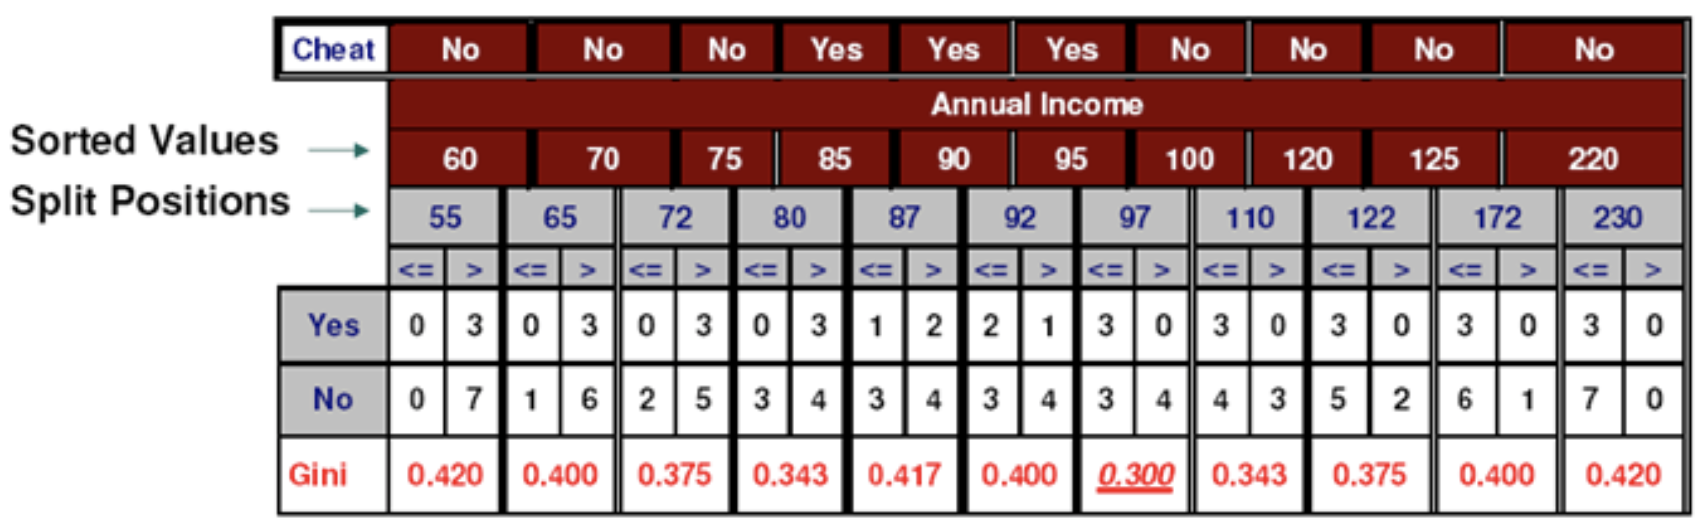
\includegraphics[scale=0.4]{figures/continuousgini.png}
    \caption{Gini Index of Continuous Attributes}
\end{figure}

\subsection{Entropy}
Entropy is a measure of the uncertainty associated with a random variable. Entropy is a splitting criterion based on information gain and measures the homogeneity of a node.

\bigskip
\begin{theo}[Entropy]{theo:theo12}
    \label{eq:entropy}
        \[
           Entropy(t) = -\sum_j^{n_c} p(j|t)\log_2 \text{ } p(j|t)
        \]
        \begin{center}
            Maximum: $(\log_2 \text{ } n_c)$ \qquad\qquad Minimum: $0.0$
        \end{center}
        Note: $p(j|t)$ is the relative frequency of class $j$ at node $t$.
\end{theo}

In the same way Gini can be used to split nodes, so can Entropy:

\bigskip
\begin{theo}[Entropy Split]{theo:theo13}
    \label{eq:entropysplit}
        \[
            GAIN_{split} = Entropy(p) - \left(\sum_{i=1}^k \frac{n_i}{n} Entropy(i)\right)
        \]
        Parent node $p$ is split into $k$ partitions.

        $n_i$ is the number of records in partition $i$
\end{theo}

The gain measures reduction in entropy achieved from the split. Choose the split that achieves the most reduction, that is, maximizes gain.
The disadvantage is that Entropy tends to prefer splits that result in a large number of partitions, each being small but pure (overfitting).
This is fixed by including the number of partitions in the equation.

\bigskip
\begin{theo}[Entropy Split Ratio]{theo:theo14}
    \label{eq:entropysplitratio}
        \[
            GainRation_{split} = \frac{Gain_{split}}{SplitInfo}
        \]
        \[
            SplitInfo = -\sum_{i=1}^k \frac{n_i}{n} \log\frac{n_i}{n}
        \]
        Parent node $p$ is split into $k$ partitions.

        $n_i$ is the number of records in partition $i$
\end{theo}

\subsection{Misclassification error}
The Classification error measures the misclassification error made by a node.

Classification error at node $t$:

\bigskip
\begin{theo}[Classification Error]{theo:theo15}
    \label{eq:classificationerror}
        \[
            Error(t) = 1-\max P(i|t)
        \]
        \begin{center}
            Maximum: $(1-\frac{1}{n_c})$ \qquad\qquad Minimum: $0.0$
        \end{center}
\end{theo}

\subsection{Comparison among Splitting Criterias}

\bigskip
\begin{figure}[H]
    \centering
    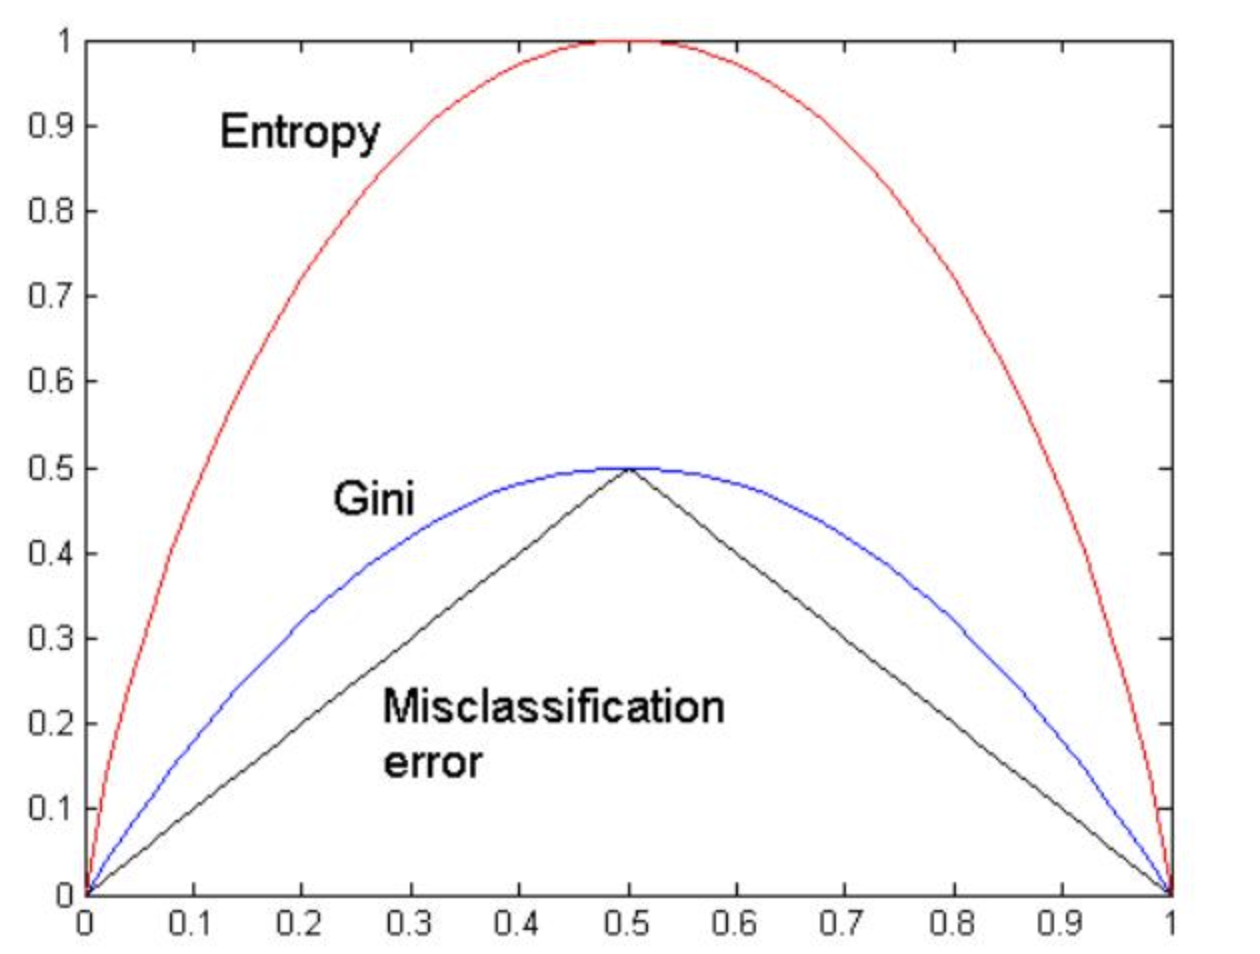
\includegraphics[scale=0.5]{figures/splittingcomparison.png}
    \caption{Splitting Criterias for a two-class problem}
\end{figure}

\section{Stopping Criteria for Tree Induction}
\begin{itemize}
    \item Stop expanding a node when all the records belong to the same class.
    \item Stop expanding a node when all the records have similar attribute values.
    \item Early termination (probably for limiting tree depth).
\end{itemize}

\section{Advantages of Decision Tree based Classification}
\begin{itemize}
    \item Inexpensive to construct.
    \item Extremely fast at classifying unknown records.
    \item Easy to interpret for small-sized trees.
    \item Accuracy is comparable to other classification techniques for many simple data sets.
\end{itemize}

\section{Classification Issues}
\subsection{Underfitting and Overfitting}
\begin{itemize}
    \item Underfitting: When a model cannot capture the underlying trend of the data. Intuitively, underfitting occurs when the model or the algorithm does not fit the data well enough. Specifically, underfitting occurs if the model or algorithm shows low variance but high bias. Underfitting is often a result of an excessively simple model. Overfitting can also arise from insufficient data points.
    \item Overfitting: When a model captures the noise of the data. Intuitively, overfitting occurs when the model or the algorithm fits the data too well. Specifically, overfitting occurs if the model or algorithm shows low bias but high variance. Overfitting is often a result of an excessively complicated model, and it can be prevented by fitting multiple models and using validation or cross-validation to compare their predictive accuracies on test data.
\end{itemize}
\bigskip
\begin{figure}[H]
    \centering
    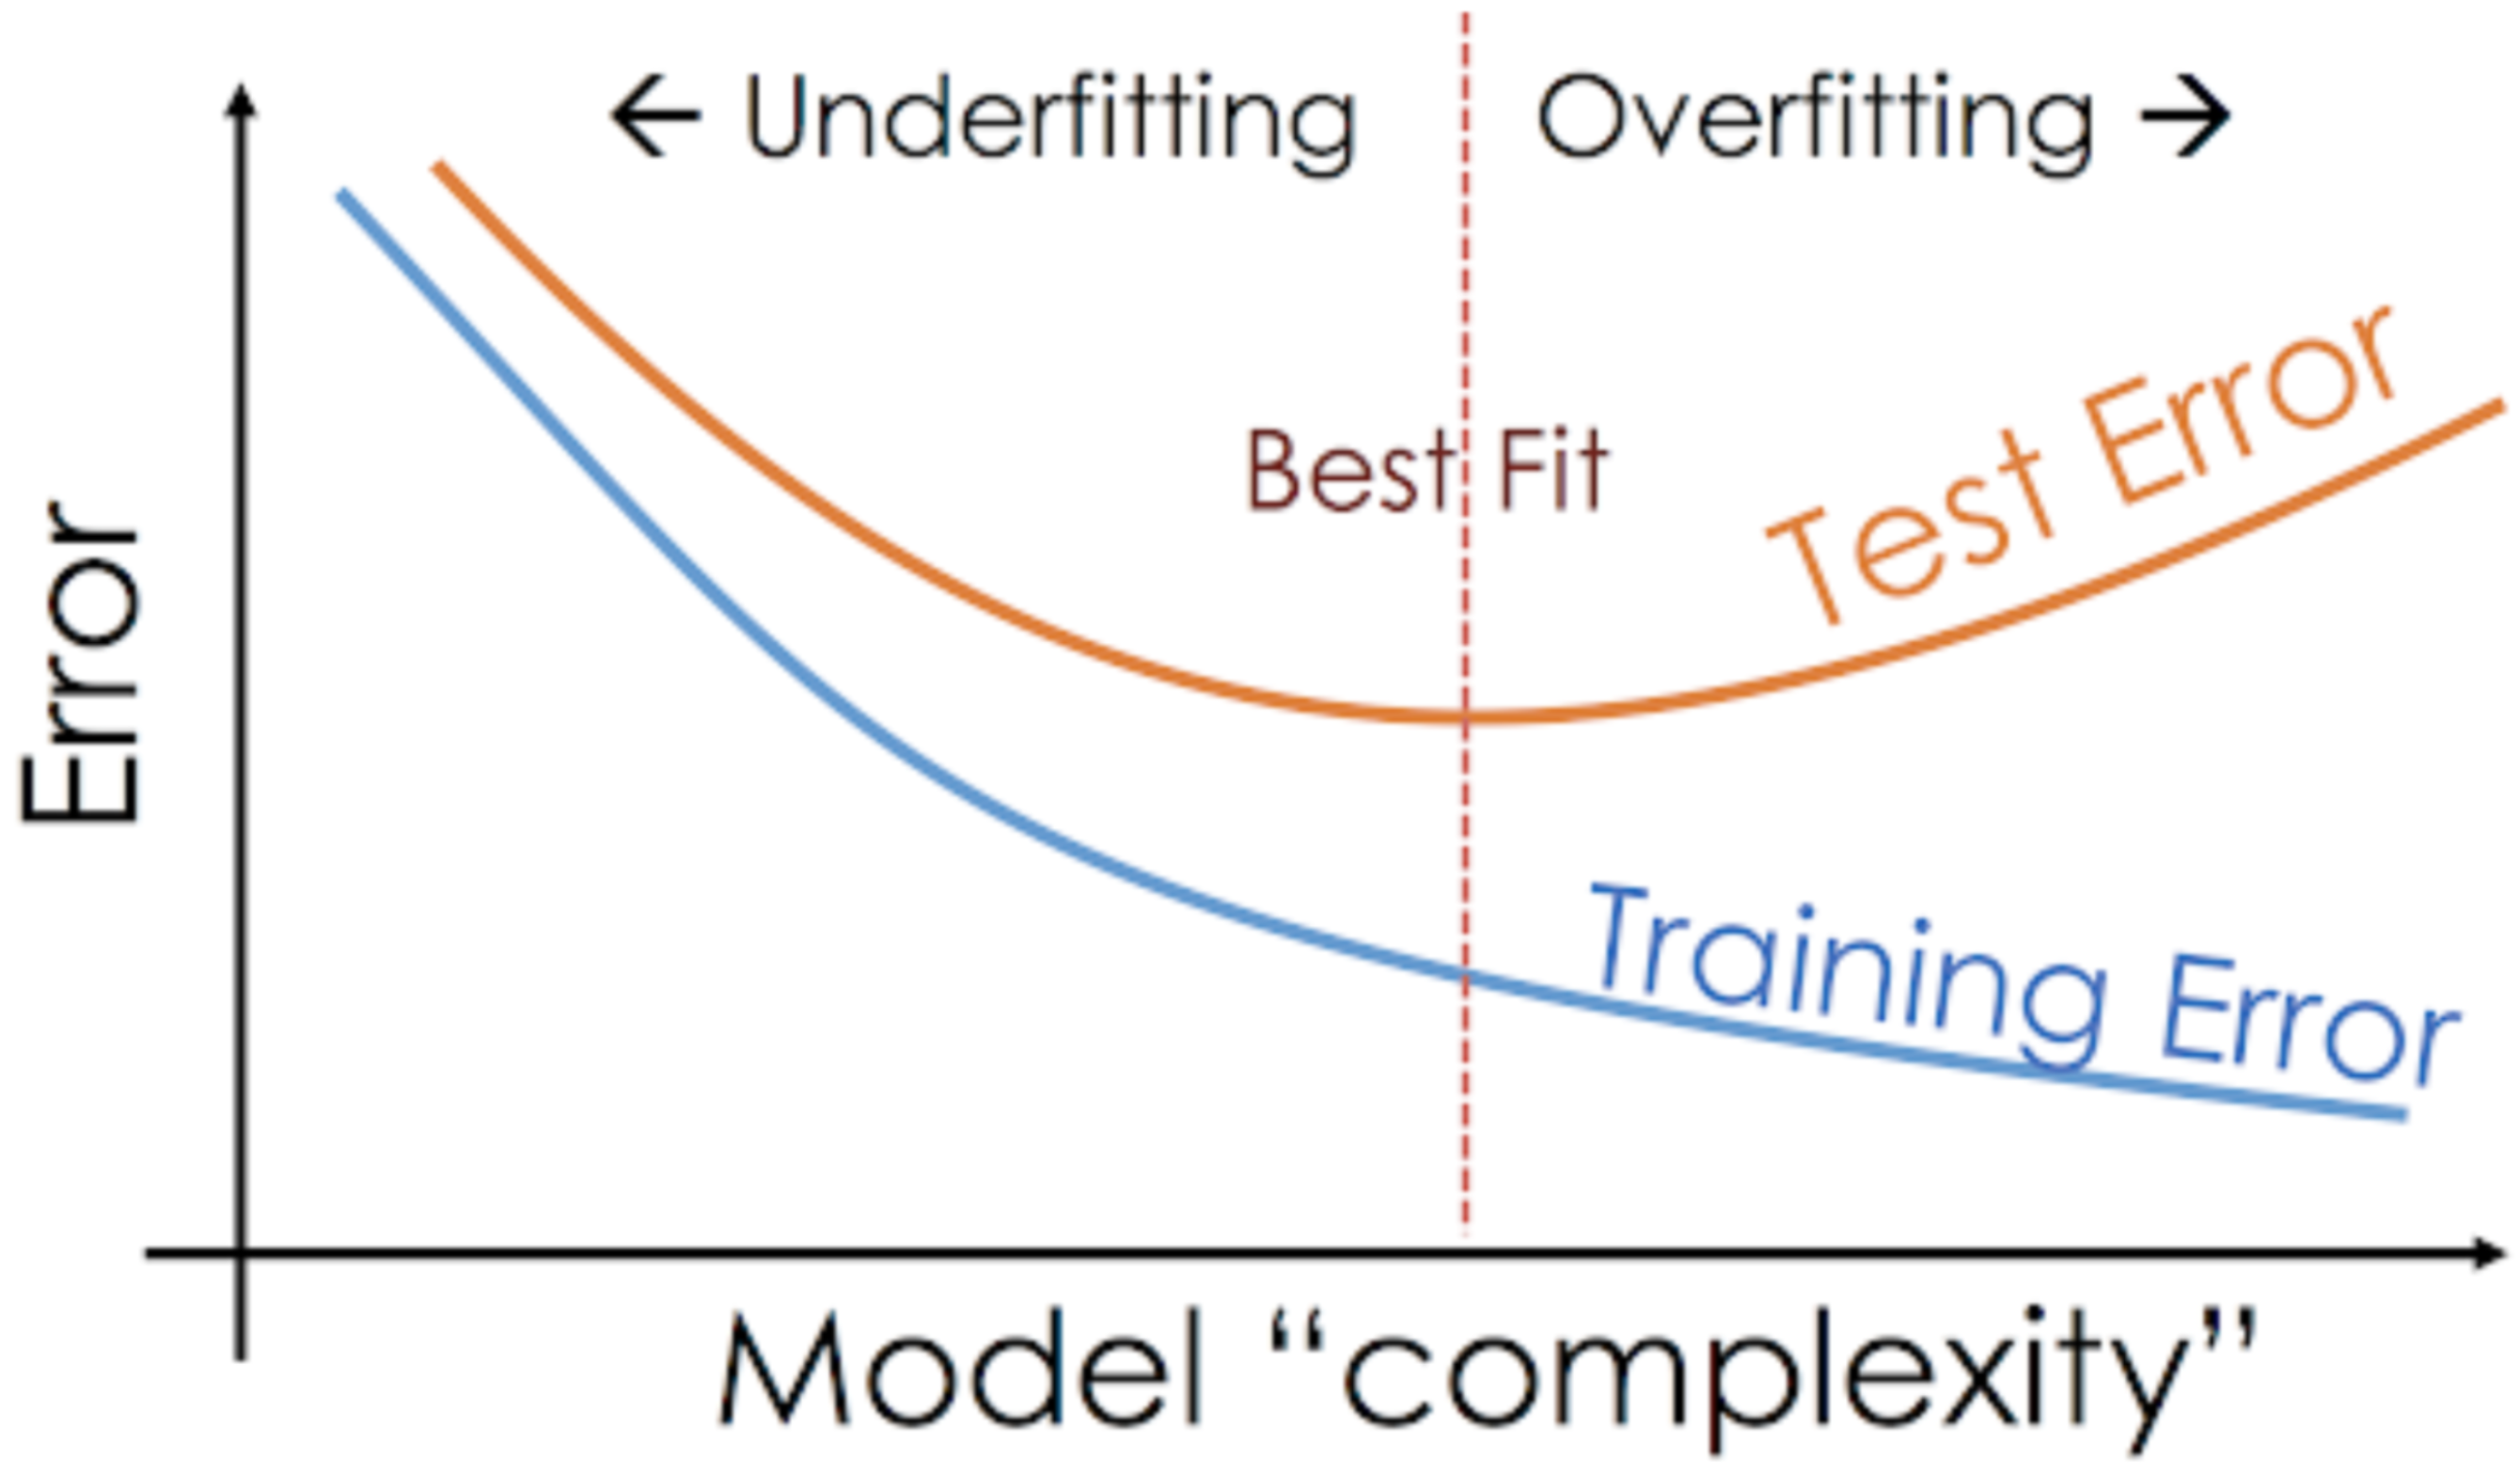
\includegraphics[scale=0.25]{figures/overunderfitting.png}
    \caption{Overfitting and underfitting}
\end{figure}

\subsection{Address Overfitting}
\subsubsection{Decision Tree Pruning}
Pre-Pruning (Early Stopping Rule):
\begin{itemize}
    \item Stop the algorithm before it becomes a fully-grown tree.
    \begin{itemize}
        \item Stop if all instances belong to the same class.
        \item Stop if all the attribute values are the same.
        \item Stop if the number of records in a node are lower than the user-specified threshold.
        \item Stop if splitting a node does not improve the impurity meassure.
    \end{itemize}
\end{itemize}

Post-Pruning:
\begin{enumerate}
    \item Grow decision tree to its entirety.
    \item Trim the nodes of the decision tree in a bottom-up fashion.
    \item If generalization error improves after trimming, replace sub-tree by a leaf node.
    \item The class label of a leaf node is determined from the majority class of instances in the sub-tree.
\end{enumerate}

\subsubsection{Occam's Razor}
\begin{itemize}
    \item Given two models of similar generalization errors, one should prefer the simpler model over the more complex model.
    \item For complex models, there is a greater chance that it was fitted accidentally by the error in data.
    \item Therefore, one should include model complexity when evaluating a model.
\end{itemize}

\subsection{Generalization Errors}
Generalization error is a measure of how accurately a model can predict outcome values for previously unseen data.
The measure is calculated from the ratio of misclassifications that can occur when choosing the majority class for all records in the node.

\begin{itemize}
    \item Training errors: Error on training ($\sum_{t=1}^n e(t)$)
    \item Generalization errors: Error on validation ($\sum_{t=1}^n e'(t)$)
\end{itemize}

Methods for estimating generalization errors:
\begin{itemize}
    \item Optimistic approach: $e'(t) = e(t)$
    \item Pessimistic approach:
    \begin{itemize}
        \item For leaf each leaf node, $e'(t_i) = e(t_i)+\frac{1}{2}$
        \item Total error: $e'(T) = e(T) + N\frac{1}{2}$ ($N$ = number of leaf nodes)
    \end{itemize}
    \item Reduced error pruning (REP)
    \begin{itemize}
        \item Uses validation data set to estimate generalization error.
    \end{itemize}
\end{itemize}

\subsection{Handling Missing Attribute Values}
Missing attribute values affect the decision tree in three major ways:
\begin{itemize}
    \item How impurity measures are computed.
    \item How to distribute instance with missing value to child nodes.
    \item How a test instance with missing value is classified.
\end{itemize}

\subsubsection{Computing Impurity Measure (Impurity Gain)}
One way of computing the information gain is as normal, without including the instances with the missing attribute.
This means that the entropy-computation for the parent is as normal, but for the children, instances with the missing attributes should be omitted, but included in the denominator. Finally, the gain is computed as normal but is multiplied by the fraction of "valid" records.

\subsubsection{Distributing Instances}
\begin{figure}[H]
    \centering
    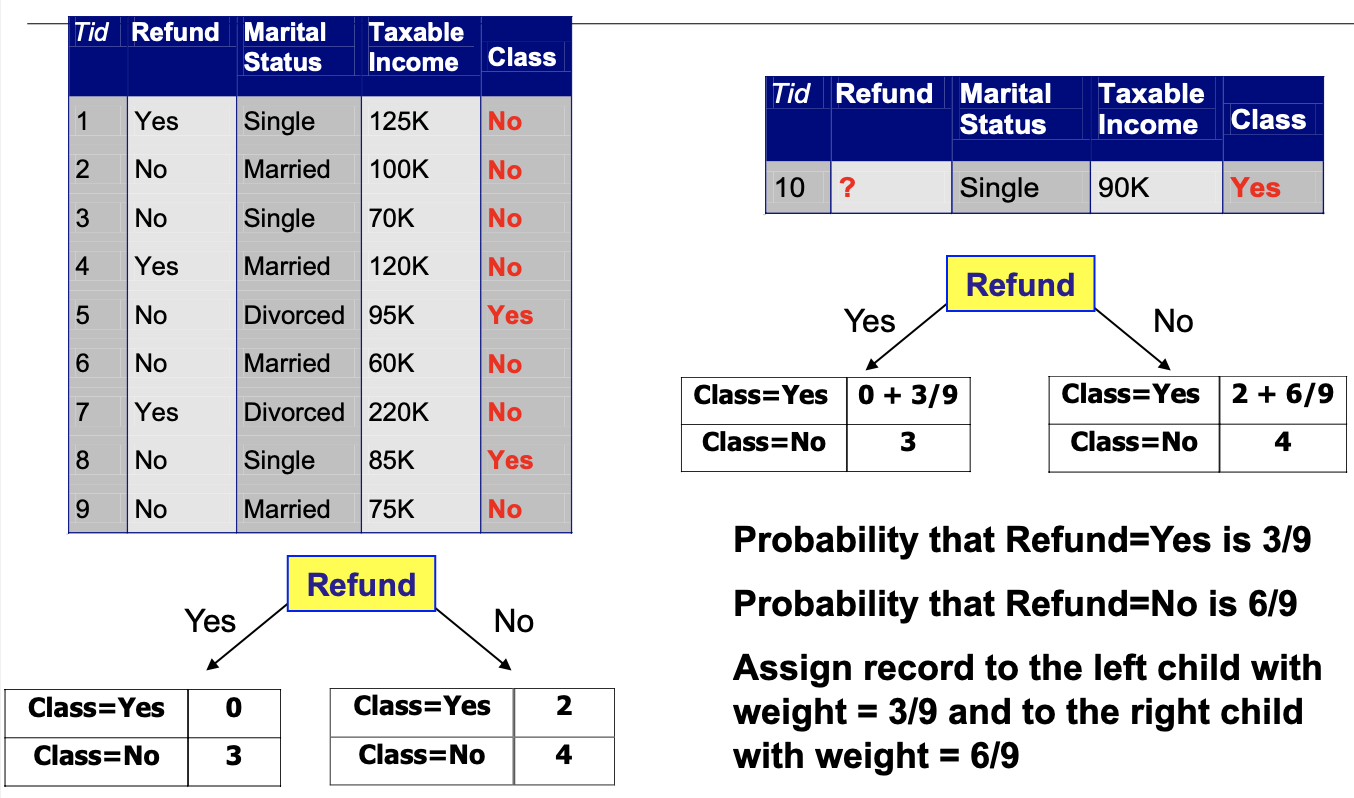
\includegraphics[scale=0.5]{figures/distributeinstances.png}
    \caption{Distributing Instances}
\end{figure}
The figure explains that since the instance with the unknown attribute corresponds to the class yes, it is distributed on both nodes, affecting the yes-class in each node.
The distribution ratio is based on the number of instances of the same class, divided by the total number of instances.

\subsubsection{Classify Instances}
To classify an instance with an unknown class, as well as having the current attribute unknown, can be done by understanding what option is more likely.
If most of the instances are of attribute 1 the instance with the unknown attribute is assumed to also have attribute 1 and follows the tree accordingly.

\subsection{Other Issues}
\subsubsection{Data Fragmentation}
\begin{itemize}
    \item The number of instances gets smaller as you traverse down the tree.
    \item Number of instances at the leaf node could be too small to make any statistically significant decision.
\end{itemize}

\subsubsection{Search Strategy}
\begin{itemize}
    \item Finding an optimal decision tree is NP-hard (exponentially).
    \item The algorithm presented so far uses a greedy, top-down, recursive partitioning strategy to induce a reasonable solution.
    \item Could use bottom-up or bi-directional algorithms.
\end{itemize}

\subsubsection{Expressiveness}
Decision trees provide expressive representation for learning discrete-valued functions, but they do not generalize well to certain types of boolean functions like parity functions.

Also, decision trees are not expressive enough for modeling continuous variables.

\subsubsection{Decision Boundary}
The borderline between two neighboring regions of different classes is known as a decision boundary.

A decision boundary is parallel to the axes because the test conditions only involve a single attribute at a time.

This could be fixed with oblique decision trees, but includes more expressive representation and can be computationally expensive.

\subsubsection{Tree Replication}
The same subtree appears in multiple branches.

